\documentclass[a4paper,10pt]{article}
\usepackage[utf8]{inputenc}
\usepackage[T1]{fontenc}
\usepackage[margin=0.75in]{geometry}
\usepackage{fancyhdr}
\usepackage{listings}
\usepackage[colorlinks]{hyperref}
\usepackage{amssymb}
% Alwayws load this last
\usepackage{xcolor}
\usepackage{soul}

\def\chpcolor{blue!60}
\def\chpcolortxt{blue!60}
\def\sectionfont{\sffamily\Large}

\setcounter{secnumdepth}{2}

\makeatletter
%Section:
\def\@sectionstrut{\vrule\@width\z@\@height12.5\p@}
\def\@makesectionhead#1{%
  {\par\vspace{20pt}%
   \parindent 0pt\raggedleft\sectionfont
   \colorbox{\chpcolor}{%
     \parbox[t]{25pt}{\color{white}\@sectionstrut\@depth4.5\p@\hfill
       \ifnum\c@secnumdepth>\z@\thesection\fi}%
   }%
   \begin{minipage}[t]{\dimexpr\textwidth-25pt-2\fboxsep\relax}
   \color{\chpcolortxt}\@sectionstrut\hspace{5pt}#1
   \end{minipage}\par
   \vspace{10pt}%
  }
}
\def\section{\@afterindentfalse\secdef\@section\@ssection}
\def\@section[#1]#2{%
  \ifnum\c@secnumdepth>\m@ne
    \refstepcounter{section}%
    \addcontentsline{toc}{section}{\protect\numberline{\thesection}\textbf{#1}}%
  \else
    \phantomsection
    \addcontentsline{toc}{section}{#1}%
  \fi
  \sectionmark{\textbf{#1}}%
  \if@twocolumn
    \@topnewpage[\@makesectionhead{#2}]%
  \else
    \@makesectionhead{\textbf{#2}}\@afterheading
  \fi
}
\def\@ssection#1{%
  \if@twocolumn
    \@topnewpage[\@makesectionhead{#1}]%
  \else
    \@makesectionhead{#1}\@afterheading
  \fi
}
\makeatother




\makeatletter
\def\@makesubsectionhead#1{%
  {\par\vspace{20pt}%
   \parindent 0pt\raggedleft\sffamily\large
   \ifnum\c@secnumdepth>\z@\color{\chpcolortxt}{\thesubsection}\fi%
   %
   \begin{minipage}[t]{\dimexpr\textwidth-2\fboxsep\relax}
   \vspace{-10pt}\color{black}\hspace{5pt}#1
   \end{minipage}\\[-10pt]
   \noindent\rule{\textwidth}{1pt}\par
   \vspace{10pt}%
  }
}
\def\subsection{\@afterindentfalse\secdef\@subsection\@ssection}
\def\@subsection[#1]#2{%
  \ifnum\c@secnumdepth>\m@ne
    \refstepcounter{subsection}%
    \addcontentsline{toc}{subsection}{\protect\numberline{\thesubsection}\textbf{#1}}%
  \else
    \phantomsection
    \addcontentsline{toc}{subsection}{\textbf{#1}}%
  \fi
  \sectionmark{\textbf{#1}}%
  \if@twocolumn
    \@topnewpage[\@makesubsectionhead{\textbf{#2}}]%
  \else
    \@makesubsectionhead{\textbf{#2}}\@afterheading
  \fi
}
\def\@ssection#1{%
  \if@twocolumn
    \@topnewpage[\@makesubsectionhead{\textbf{#1}}]%
  \else
    \@makesubsectionhead{\textbf{#1}}\@afterheading
  \fi
}
\makeatother



\definecolor{codegreen}{rgb}{0,0.6,0}
\definecolor{codegray}{rgb}{0.5,0.5,0.5}
\definecolor{codepurple}{rgb}{0.58,0,0.82}
\definecolor{backcolour}{rgb}{0.95,0.95,0.92}

%Code listing style named "mystyle"
\lstdefinestyle{mystyle}{
  backgroundcolor=\color{backcolour},   commentstyle=\color{codegreen},
  keywordstyle=\color{magenta},
  numberstyle=\tiny\color{codegray},
  stringstyle=\color{codepurple},
  basicstyle=\ttfamily\footnotesize,
  breakatwhitespace=false,         
  breaklines=true,                 
  captionpos=b,                    
  keepspaces=true,                 
  numbers=left,                    
  numbersep=5pt,                  
  showspaces=false,                
  showstringspaces=false,
  showtabs=true,                  
  tabsize=2
}

%"mystyle" code listing set
\lstset{style=mystyle}


\newcommand{\xhdr}[1]{\vspace{5pt}\noindent{\color{blue!60}\textbf{#1}}}


\newcommand{\task}[1]{\xhdr{ {\large $\mathbf{\blacktriangleright}$} \texttt{TASK #1}}}


\usepackage{tcolorbox}
\newtcolorbox{taskbox}{
    arc=0pt,
    boxrule=1pt,
    colback=gray!10,
    colframe=blue!60,
    width=\textwidth,
    halign=left,
}
\usepackage{tikz}
\usetikzlibrary{automata, positioning, arrows}






\begin{document}
\tikzset{
->, % makes the edges directed
>=stealth, % makes the arrow heads bold
node distance=2cm, % specifies the minimum distance between two nodes. Change if necessary.
every state/.style={thick, fill=gray!10}, % sets the properties for each ’state’ node
initial text=$ $, % sets the text that appears on the start arrow
}

\sffamily

\begin{center}
\noindent\rule{\textwidth}{1pt}\\[10pt]
{\color{blue!60}{AI539 Natural Language Processing with Deep Learning -- Homework 2}}\\[10pt]
{\LARGE Recurrent Neural Networks and Sentence Representations}\\[10pt]
\noindent\rule{\textwidth}{1pt}
\end{center}

\noindent\textbf{Overview and Objectives.} In this homework, we'll get more familiar with LSTMs by doing a bit of math, interacting with simple versions in toy settings, and then move on to developing a full pipeline for part-of-speech tagging in English with a Bidirectional LSTM.\\

\noindent\textbf{How to Do This Assignment.} The assignment walks you through completing the provided skeleton code and analyzing some of the results. Anything requiring you to do something is marked as a "Task" and has associated points listed with it. You are expected to turn in both your code and a write-up answering any task that requested written responses. Submit a zip file containing your completed skeleton code and a PDF of your write-up to Canvas.\\ 

\noindent\textbf{Advice.} Start early. Students will need to become familiar with \texttt{pytorch} for this and future assignments. Extra time may be needed to get used to working remotely on the GPU cluster here. You can also use GPU-enabled runtimes in Colab \url{colab.research.google.com}.

\section{Demystifying Recurrent Neural Networks [5pt]}

\subsection{Hand Designing A Network for Parity}

Consider a univariate LSTM defined given the following equations. We refer to this model as univariate because all inputs, outputs, and weights are scalars. $\sigma(\cdot)$ is a sigmoid activation. 
\begin{eqnarray}
    i_t &=& \sigma(w_{ix}x_t + w_{ih}h_{t-1}+b_i)\\
    f_t &=& \sigma(w_{fx}x_t + w_{fh}h_{t-1}+b_f)\\
    o_t &=& \sigma(w_{ox}x_t + w_{oh}h_{t-1}+b_o)\\
    g_t &=& \tanh(w_{gx}x_t + w_{gh}h_{t-1}+b_g)\\
    c_t &=& f_tc_{t-1}+i_tg_t\\
    h_t &=& o_t \tanh(c_t)
\end{eqnarray}

\noindent To ground this complicated looking model, we will consider a simple sequence classification problem -- parity of binary strings. Given an arbitrarily-long binary string $b \in \{0,1\}^*$, classify whether it has an even or odd number of ones. For example all these strings have an even parity -- \texttt{``~~'', 0000, 101101} -- and these an odd parity -- \texttt{1, 0011001, 00011100}. Below is a simple DFA\footnote{\url{https://en.wikipedia.org/wiki/Deterministic_finite_automaton}} that accepts strings with odd parity at the accepting state $s_2$. As it only has two states, it seems solving the parity classification problem only requires storing 1 bit of information in memory.
\begin{center}
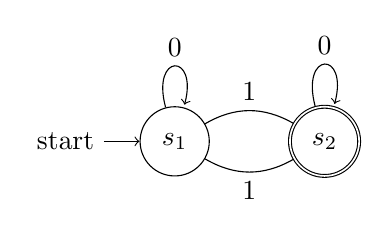
\begin{tikzpicture}
\node[state, initial] (q1) {$s_1$};
\node[state, accepting,right = of q1] (q2) {$s_2$};
\draw (q1) edge[loop above] node{0} (q1)
(q1) edge[bend left, above] node{1} (q2)
(q2) edge[bend left, below] node{1} (q1)
(q2) edge[loop above] node{0} (q2);
\end{tikzpicture}
\end{center}

\noindent Another way to think about this computation is as a recursive application of \texttt{XOR} over time. If the parity up to element $t-1$ is 1 (odd) and we see a 1 for element $t$, the updated parity is $1~\mbox{XOR}~1 = 0$ (even). Likewise, if at time $t+1$ we observe another $1$, $0~\mbox{XOR}~1 = 1$. In other words, $\mbox{PARITY}(X,t) = X[t]~\mbox{XOR PARITY}(X, t-1)$ and $\mbox{PARITY}(X, -1)=0$ by definition. This sounds like the sort of operation we can do with an LSTM!




\vspace{5pt}
\begin{taskbox}
\task{1.1 [5 pt]} Manually find weights and biases for the univariate LSTM defined above such that the final hidden state will be greater than or equal to 0.5 for odd parity strings and less than 0.5 for even parity. The parameters you must provide values for are $w_{ix}$, $w_{ih}$, $b_i$, $w_{fx}$, $w_{fh}$, $b_f$, $w_{ox}$, $w_{oh}$, $b_o$, $w_{gx}$, $w_{gh}$, $b_g$ and are all scalars. The LSTM will take one bit of the string (0 or 1) as input $x$ at each time step. A tester is set up in \texttt{univariate\_tester.py} where you can enter your weights and check performance. \\[5pt]

\emph{Hints: Some of the weights will likely be zero. Others may be large. Scale matters, larger weights will saturate the activation functions. Also note that \texttt{A XOR B} can be written as \texttt{(A OR B) AND (A NAND B)}. Work backwards and try to find where this sort of two-term structure could be implemented.} 

\end{taskbox}
\vspace{5pt}

\noindent Through this exercise, we've shown that a 1-dimensional LSTM \emph{is sufficient to solve parity of binary strings of arbitrary length.} In the next section, we'll try to actually train an LSTM for this task. Hint: It may be harder than you think.



\section{Learning to Copy Finite State Machines [10pt]}

Let's probe LSTMs a bit by making them mimic simple finite state machines. The rest of this assignment will work within the PyTorch deep learning framework. You'll need to install PyTorch in your development environment. 



\subsection{Parity: Examining Generalization To Longer Sequences}
First, lets try to train an LSTM to perform the parity task we just did manually. The \texttt{driver\_parity.py} file provide skeleton code for these experiments including a parity dataset shown below. During training, it generates all binary strings of length 0 to \texttt{max\_length}. At inference, it generates all binary strings of length \texttt{max\_length}.

\begin{center}
\begin{minipage}{0.8\textwidth}
\begin{lstlisting}[language=Python, caption=Parity Dataset]
class Parity(Dataset):

    def __init__(self,split="train", max_length=4):
      if split=="train":
        self.data = []
        for i in range(1,max_length+1):
          self.data += [torch.FloatTensor(seq) for seq in itertools.product([0,1], repeat=i)]
      else:
        self.data = [torch.FloatTensor(seq) for seq in itertools.product([0,1], repeat=max_length)]

    def __len__(self):
        return len(self.data)

    def __getitem__(self, idx):
        x = self.data[idx]
        y = x.sum() % 2
        return x,y 
\end{lstlisting}
\end{minipage}
\end{center}

\noindent To train our network, we can build a DataLoader from our Parity dataset (see below). However, our dataset contains strings of variable length so we need to pass a custom function to our data loader describing how to combine elements in a sampled batch together.


\begin{center}
\begin{minipage}{0.8\textwidth}
\begin{lstlisting}[language=Python, caption=Data loader]
    train = Parity(split='train', max_length=max_length)
    train_loader = DataLoader(train, batch_size=B, shuffle=True,
                                collate_fn=pad_collate)
\end{lstlisting}
\end{minipage}
\end{center}

\noindent Our \texttt{pad\_collate} function puts all the elements of a batch in a $B \times T_{\mbox{max}}$ tensor for inputs and a $B$ tensor for outputs where $T_{\mbox{max}}$ is the largest length in the batch. Shorter sequences are zero-padded. A batch of inputs looks like: 

\begin{center}
\begin{minipage}{0.8\textwidth}
\begin{lstlisting}[language=Python, caption=Example input for a batc]
    tensor([[1., 1., 0., 0., 0.],
            [0., 1., 0., 1., 0.],
            [0., 0., 0., 0., 0.],
            [0., 1., 1., 0., 1.],
            [0., 1., 1., 0., 0.]], device='cuda:0')
\end{lstlisting}
\end{minipage}
\end{center}




\vspace{5pt}
\begin{taskbox}
\task{2.1 [5 pt]} Implement the \texttt{ParityLSTM} class in \texttt{driver\_parity.py}. Your model's \texttt{forward} function should process the batch of binary input strings and output a $B \times 2$ tensor $y$ where $y_{b,0}$ is the score for the $b^{th}$ element of the batch having an even parity and $y_{b,1}$ for odd parity. You may use any PyTorch-defined LSTM functions. Larger hidden state sizes will make for easier training in my experiments. Running \texttt{driver\_parity.py} will train your model and output per-epoch training loss and accuracy. A correctly-implemented model should approach 100\% accuracy on the training set. In your write-up for this question, describe any architectural choices you made.\\[5pt]

\emph{Hint: Efficiently processing batches with variable input lengths requires some bookkeeping or else the LSTM will continue to process the padding for shorter sequences along with the content of longer ones. See pack\_padded\_sequence and pad\_packed\_sequence documentation in PyTorch.}
\end{taskbox}
\vspace{5pt}


\vspace{5pt}
\begin{taskbox}
\task{2.2 [1 pt]} \texttt{driver\_parity.py} also evaluates your trained model on binary sequences of length 0 to 20 and saves a corresponding plot of accuracy vs.~length. Include this plot in your write-up and describe the trend you observe. Why might the model behave this way?
\end{taskbox}
\vspace{5pt}

\vspace{5pt}
\begin{taskbox}
\task{2.3 [3 pt]} We know from 1.1 that even a univariate LSTM (one with a scalar hidden state) can theoretically solve this problem. Run a few (3-4) experiments with different hidden state sizes, what is the smallest size for which you can still train to fit this dataset? Feel free to adjust any of the hyper-parameters in the optimization in the \texttt{train\_model} function if you want. Describe any trends you saw in training or the generalization experiment as you reduced the model capacity.\\[5pt]

\emph{Note: In developing this assignment, I never successfully got it down to a hidden dimension of 1. Lower dimensional settings tended to be sensitive to batch size and learning rate. Don't spend all night tuning this unless you've finished the rest of the assignment and have nothing better to do.}
\end{taskbox}
\vspace{5pt}

\subsection{Embedded Reber Grammars: Thinking About Memory}
Next we turn to recognizing an Embedded Reber Grammar (ERG). An ERG generation diagram is shown below. To generate an ERG string, start from the leftmost black node and sample any outgoing edge (only B in this case) and write down the letter of that edge. Repeat this process from the new node until reaching the right-most black node through the edge labelled E. So \texttt{BTBTSSXSETE} is a valid ERG string. Notice that the sub-networks in dashed boxes are identical for the upper and lower branch. These are the Reber Grammars that are embedded in this larger grammar. To make longer strings, the dashed boxes can be repeated $k$ times (E edge returns to start) before exiting to the T/P edges headed towards the terminal node on the right.

\begin{center}
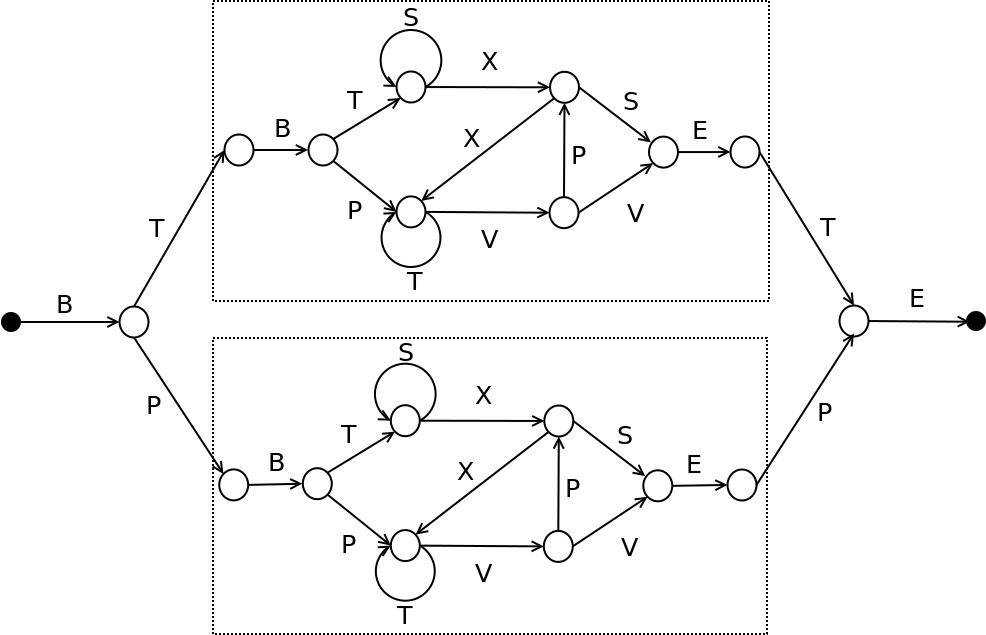
\includegraphics[width=0.49\textwidth]{figures/EmbeddedReber.png}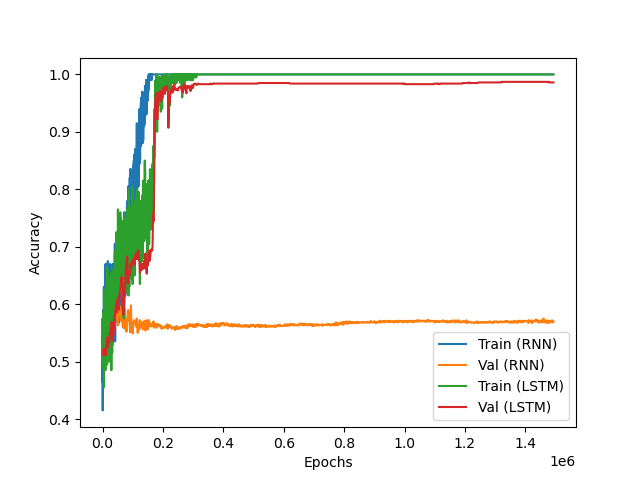
\includegraphics[width=0.49\textwidth]{figures/reber_generalization.png}
\end{center}

\noindent The plot on the right shows train and validation accuracy over training for an LSTM and vanila RNN on the task of identifying ERG strings with $k=4$. An example string from this grammar is \texttt{BTBTXSEBTXSEBPVVEBTXXVVETE}. Breaking it out, its easy to see the structure -- \texttt{BT} \texttt{BTXSE} \texttt{BTXSE} \texttt{BPVVE}
\texttt{BTXXVVE}
\texttt{TE} -- as a prefix, four repeated Reber Grammar strings, and a suffix. The dataset contained 50\% positives samples, 25\% negative with a random perturbation of one character, and 25\% negatives with the second-to-last letter perturbed. In this setting, the vanilla RNN model overfit to the training set given sufficient time, but failed to generalize. In contrast, the LSTM model generalized well to the test set.

\vspace{5pt}
\begin{taskbox}
\task{2.4 [1 pt]} It has been demonstrated that vanilla RNNs have a hard time learning to classify whether a string was generated by an ERG or not. LSTMs on the other hand seem to work fine. Based on the structure of the problem and what you know about recurrent networks, why might this be the case? 
\end{taskbox}
\vspace{5pt}

\section{Part-of-Speech Tagging [15pt]}
Now lets get to work on a real problem -- part-of-speech tagging in English. This is a many-to-many sequence problem where each word in an input must be labelled with a corresponding part-of-speech tag. The goal of this section will be to train a bidirectional LSTM model for this task. Unlike in the previous sections, no skeleton code will be provided and students are responsible for building the whole pipeline including text processing, data loading, model design, training, and evaluation. Feel free to use any libraries you wish to accomplish this.

We will be using the Universal Dependencies\footnote{https://universaldependencies.org/} English Part-Of-Speech (UDPOS) benchmark. The easiest way to load this dataset is through the \texttt{torchtext} module. The code below loads the dataset and prints out an example. 


\begin{center}
\begin{minipage}{0.8\textwidth}
\begin{lstlisting}[language=Python, caption=Loading the UD En POS benchmark]
from torchtext import data
from torchtext import datasets
TEXT = data.Field(lower = True)
UD_TAGS = data.Field(unk_token = None)
fields = (("text", TEXT), ("udtags", UD_TAGS))
train_data, valid_data, test_data = datasets.UDPOS.splits(fields)

def visualizeSentenceWithTags(example):
  print("Token"+"".join([" "]*(15))+"POS Tag")
  print("---------------------------------")
  for w, t in zip(example['text'], example['udtags']):
    print(w+"".join([" "]*(20-len(w)))+t)

\end{lstlisting}
\end{minipage}
\end{center}


\begin{center}
\begin{minipage}{0.8\textwidth}
\begin{lstlisting}[language=Python, caption=Visualizing a sentence and its associated list of tags.]

> visualizeSentenceWithTags(vars(train_data.examples[997]))
Token               POS Tag
---------------------------------
they                PRON
are                 AUX
doing               VERB
it                  PRON
deliberately        ADV
.                   PUNCT
\end{lstlisting}
\end{minipage}
\end{center}

\noindent Notice that there is a train, validation, and test split of the dataset. We should only evaluate on test once when we are completely done tuning our model on validation and are looking to report final results. 

\vspace{5pt}
\begin{taskbox}
\task{3.1 [2 pt]} The first step for any machine learning problem is to get familiar with the dataset. Read through random samples of the dataset and summarize what topics it seems to cover. Also look at the relationship between words and part-of-speech tags -- what text preprocessing would be appropriate or inappropriate for this dataset? Produce a histogram of part-of-speech tags in the dataset -- is it balanced between all tags? What word-level accuracy would a simple baseline that  picked the majority label achieve?
\end{taskbox}
\vspace{5pt}


You will need to get the dataset into a form that we can use in a model -- i.e.~numeralized batches of sequences and their labels. Simple examples of dataset classes and dataloaders that rely on our Vocabulary code from last assignment have been demonstrated in lecture. Another option is to look into the \texttt{torchtext.data} APIs which can flexibly handle text datasets like this one and take care of tokenization / numeralization with less effort -- provided you spend the time learning the API. Either way is fine for this assignment.

The next step is to implement your model and the training routine. The lectures and other skeleton code in this assignment should provide a good starting point for these. If you run into trouble, printing out the shapes of tensors and reading the PyTorch documentation can be very helpful. A useful development strategy is to operate only on a single batch at first -- if your model can't quickly fit the batch, something is wrong. Once you get a basic model running, you'll want to tune parameters and network structure to achieve good validation accuracy. 

\vspace{5pt}
\begin{taskbox}
\task{3.2 [10 pt]} Create a file \texttt{driver\_udpos.py} that implements and trains a bidirectional LSTM model on this dataset with cross entropy loss. The BiLSTM should predict an output distribution over the POS tags for each token in a sentence. In your written report, produce a graph of training and validation loss over the course of training. Your model should be able to achieve >70\% per-word accuracy fairly easily. \\[5pt] 

To achieve stronger performance, you will likely need to tune hyper-parameters or model architecture to achieve lower validation loss. Using pretrained word vectors will likely help as well. You may also wish to employ early-stopping -- regularly saving the weights of your model during training and then selecting the saved model with the lowest validation loss. In your report, describe any impactful decisions during this process. Importantly -- \texttt{DO NOT EVALUATE ON TEST DURING THIS TUNING PROCESS}.\\[5pt]

Once you are done finetuning, evaluate on the test split of the data and report the per-word accuracy. 
\end{taskbox}
\vspace{5pt}

\vspace{5pt}
\begin{taskbox}
\task{3.3 [3 pt]} Implement a function \texttt{tag\_sentence(sentence, model)} that processes an input sentence (a string) into a sequence of POS tokens. This will require you to tokenize/numeralize the sentence, pass it through your network, and then print the result. Use this function to tag the following sentences:\\[5pt]

The old man the boat.

The complex houses married and single soldiers and their families.

The man who hunts ducks out on weekends.


\end{taskbox}
\vspace{5pt}

%\section{Additional Resources}
\vspace{20pt}
\renewcommand{\section}[2]{ {\hspace{-20pt}\color{blue!60}{\Large #2}} }

%\bibliography{refs}
%\bibliographystyle{ieeetr}
    
\end{document}
